\documentclass[journal]{vgtc}                % final (journal style)
%\documentclass[review,journal]{vgtc}         % review (journal style)
%\documentclass[widereview]{vgtc}             % wide-spaced review
%\documentclass[preprint,journal]{vgtc}       % preprint (journal style)
%\documentclass[electronic,journal]{vgtc}     % electronic version, journal

%% Uncomment one of the lines above depending on where your paper is
%% in the conference process. ``review'' and ``widereview'' are for review
%% submission, ``preprint'' is for pre-publication, and the final version
%% doesn't use a specific qualifier. Further, ``electronic'' includes
%% hyperreferences for more convenient online viewing.

%% Please use one of the ``review'' options in combination with the
%% assigned online id (see below) ONLY if your paper uses a double blind
%% review process. Some conferences, like IEEE Vis and InfoVis, have NOT
%% in the past.

%% Please note that the use of figures other than the optional teaser is not permitted on the first page
%% of the journal version.  Figures should begin on the second page and be
%% in CMYK or Grey scale format, otherwise, colour shifting may occur
%% during the printing process.  Papers submitted with figures other than the optional teaser on the
%% first page will be refused.

%% These three lines bring in essential packages: ``mathptmx'' for Type 1
%% typefaces, ``graphicx'' for inclusion of EPS figures. and ``times''
%% for proper handling of the times font family.

\usepackage{natbib}
\usepackage{mathptmx}
\usepackage{graphicx}
\usepackage{times}

%% We encourage the use of mathptmx for consistent usage of times font
%% throughout the proceedings. However, if you encounter conflicts
%% with other math-related packages, you may want to disable it.

%% If you are submitting a paper to a conference for review with a double
%% blind reviewing process, please replace the value ``0'' below with your
%% OnlineID. Otherwise, you may safely leave it at ``0''.
\onlineid{0}

%% declare the category of your paper, only shown in review mode
\vgtccategory{Research}

%% allow for this line if you want the electronic option to work properly
\vgtcinsertpkg

%% In preprint mode you may define your own headline.
%\preprinttext{To appear in an IEEE VGTC sponsored conference.}

%% Paper title.

\title{Graphical Tests for Power Comparison of Competing Designs}

%% This is how authors are specified in the journal style

%% indicate IEEE Member or Student Member in form indicated below
\author{Lendie Follett, Heike Hofmann, Mahbub Majumder, Dianne Cook}
\authorfooter{
%% insert punctuation at end of each item
\item
 Lendie Follett is a graduate student in Statistics at Iowa State University, E-mail: lfollett@iastate.edu.
\item
everybody else is at Iowa State University, too
}

%other entries to be set up for journal
\shortauthortitle{Follett \MakeLowercase{\textit{et al.}}: Comparison of Competing Layouts}
%\shortauthortitle{Firstauthor \MakeLowercase{\textit{et al.}}: Paper Title}

%% Abstract section.
\abstract{
Lineups  \cite{buja:2009, wickham:2010} have been established as tools for visual testing
similar to standard statistical inference tests, allowing us to
evaluate the validity of graphical findings in an objective manner. In
simulation studies  \cite{majumder:2011} lineups have been shown as being efficient: the
power of visual tests is comparable to classical tests while being
much less stringent in terms of distributional assumptions made. This
makes lineups versatile, yet powerful, tools in situations where
conditions for regular statistical tests are not or cannot be met. In
this paper we introduce lineups as a tool for evaluating the power of
competing graphical designs. We highlight some of the theoretical
properties and then show results from two studies evaluating competing
designs: both studies are designed to go to the threshold of our
perceptual abilities to highlight differences between designs. We use
both accuracy and speed of evaluation as measures of a successful
design. The first study compares the choice of coordinate system:
polar versus Euclidean coordinates. The results show strong support in
favor of Euclidean coordinates in finding fast and accurate answers to
spotting patterns. The second study is aimed at finding shift
differences between distributions. Both studies are motivated by data
problems that we have recently encountered, and explore using
simulated data to evaluate the plot designs under controlled
conditions.  Amazon Turk is used to conduct the studies.  The lineups
provide an effective mechanism for objectively evaluating plot
designs.
} % end of abstract

%% Keywords that describe your work. Will show as 'Index Terms' in journal
%% please capitalize first letter and insert punctuation after last keyword
\keywords{Lineups, visual inference, Power Comparison, Efficiency of Displays.}

%% ACM Computing Classification System (CCS). 
%% See <http://www.acm.org/class/1998/> for details.
%% The ``\CCScat'' command takes four arguments.

\CCScatlist{ % not used in journal version
  \category{H.5.2}{Information Interfaces and Presentation}{ User Interfaces --- Graphical user interfaces (GUI), Interaction styles, Screen design, Evaluation/methodology}
  \CCScat{I.6.8}{Computing Methodologies}%
  {Simulation and Modeling}{Visual Simulation};
}

\graphicspath{{images/}}

%% Uncomment below to include a teaser figure.
\teaser{
\centering
\includegraphics[height=1in]{polar}
\includegraphics[height=1in]{eucline}
%\includegraphics[width=16cm]{CypressView.eps}
\caption{teaser chart should include all different designs}
}

%% Uncomment below to disable the manuscript note
%\renewcommand{\manuscriptnotetxt}{}

%% Copyright space is enabled by default as required by guidelines.
%% It is disabled by the 'review' option or via the following command:
% \nocopyrightspace

%%%%%%%%%%%%%%%%%%%%%%%%%%%%%%%%%%%%%%%%%%%%%%%%%%%%%%%%%%%%%%%%
%%%%%%%%%%%%%%%%%%%%%% START OF THE PAPER %%%%%%%%%%%%%%%%%%%%%%
%%%%%%%%%%%%%%%%%%%%%%%%%%%%%%%%%%%%%%%%%%%%%%%%%%%%%%%%%%%%%%%%%

\begin{document}

%% The ``\maketitle'' command must be the first command after the
%% ``\begin{document}'' command. It prepares and prints the title block.

%% the only exception to this rule is the \firstsection command
\firstsection{Introduction}

\maketitle

%% \section{Introduction} %for journal use above \firstsection{..} instead
%We introduce and discuss a tool for comparing different charts that are renderings of the same data in order to evaluate them for efficiency.
We would like to display data so that the information it contains is relayed in the most efficient way. There are many methods when it comes to how the data can be displayed but the varying efficiency of these methods is hard to measure and compare. We are using different renderings of the  same data in order to evaluate designs for their efficiency by measuring how accurately and quickly viewers can extract pieces of information. 
This is a technique that has been used for many years now, starting possibly with the (convenience) study on evaluating difficulty of a set of different visual tasks by \citet{cleveland:1984}, which has recently been repeated finding similar results based on a larger and more representative study by \citet{kosara:2010}.

XXX What do we differently? We use lineup charts.
XXX Why is that better? 
Usually, we need simulation studies to be able to completely control for the signal strength in the data. For charts, this is unrealistic. The need for displaying information particularly efficiently or accurately generally arises from the setting that we are exploring a data set and trying to learn new insight from it. Often, it is difficult at best to come close to a particular data situation using simulated data, which makes studies on competing  designs find answers to the wrong questions.

As designers of charts we are guided by experience, knowledge of perceptual strengths and weaknesses, and aesthetic preferences. It is impossible to make the final decision on the design in an  objective manner.
Lineup tests allow us to directly use the data at hand to evaluate different competing designs by using permutations tests \cite{good:2011} of the original dataset.

A simulation study might not be completely 

Introduce lineup charts \citep{buja:2009}. Include power discussion.


\section{Experimental Setup}
Describe the experimental setup: polar charts versus euclidean - with and without reference lines.
Figure showing all four types using the same dataset. 
Discuss construction of each one. Discuss construction of null chart.

The goal of this experiment is to understand the efficiency of displaying information using euclidian and polar coordinates. Efficiency is the deviation from independence, which can be simulated by taking permutations of the original dataset. Data concerning wind patterns and time between flights at SEA airport is used for these charts. The lineup chart is composed of 20 graphics with all of the exact same characteristics except for the data. One of the 20 graphics will be using original airport data while the other 19 will be permutations of that data. There are other variables which are introduced to further our understanding of the way we perceive euclidian and polar coordinates. All combinations of each level of the variables are involved in the experiment for both polar and euclidian coordinates. The graphics in each chart will all have exactly the same level of the variables with the only difference being the data. 

It is possible that one of the chart types benefits more from additional components such as reference lines. The polar and euclidian null charts will be shown either with or without a white reference line. The line is placed at slightly over 50 percent of the y axis.

 The x-axis has four placements. The original dataset contains a characteristic wave pattern, which for euclidian coordinates, may be a large factor contributing to the perceived effectiveness of the graphic. Characteristic patterns such as the wave pattern may be perceived in a different way when viewed in polar coordinates. When the x-axis is is shifted the look of the pattern changes. The wave pattern is broken up for euclidian coordinates but for polar coordinates is only shifted around the axis. 

Amount of information necessary for detection as well as correctness is measure for efficiency of chart so the sample size which was taken from the original dataset is of interest. The original data set contained XXX,XXX observations from which we sampled 2, 4, 6, 8, 10, and 24 percent. Samples of 2, 4, and 6 percent were repeated twice to gain more information about the effectiveness of the charts at these levels. Small sample sizes are easier to obtain because of time and money constraints, as well as others. It would be nice to know if there is one type of chart which can show data trends using less information. 


 All combinations of these variables were repeated for plots with a reference line and without a reference line, as shown in figure \ref{layouts}.This figure shows examples of graphics showing the actual data, which in the experiment would be randomly positioned among 19 null plots. In total there are XXX unique charts which represent all different combinations of sample size, coordinate type, x-axis placement, and whether or not there is a reference line. The charts are all assigned a difficulty level, which is based on sample size, on a scale from zero to four. There are two plots assigned a difficulty level of zero. These two charts, one polar and one Euclidian, were made from computer generated data and intended to be at the level where an individual, if he or she is not purely guessing, should be able to find the correct plot. 

\begin{figure}[htbp] %  figure placement: here, top, bottom, or page
   \centering
   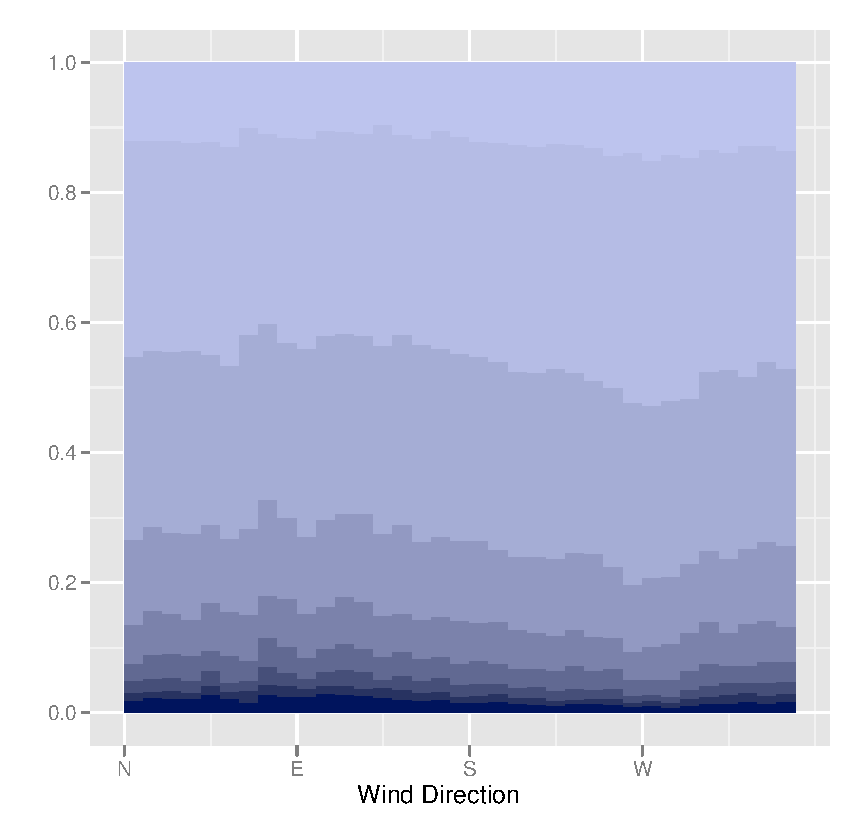
\includegraphics[width=1.3in]{Euclidian_NoLine.pdf} 
   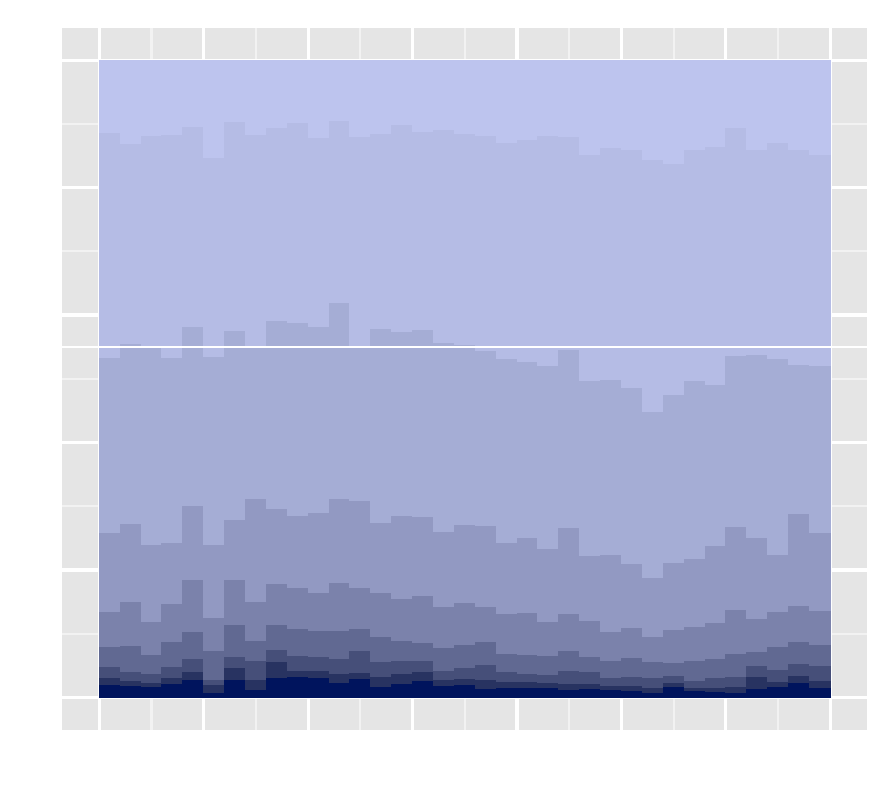
\includegraphics[width=1.3in]{Euclidian_Line.pdf} \\
   \includegraphics[width=1.3in]{Polar_NoLine.pdf} 
   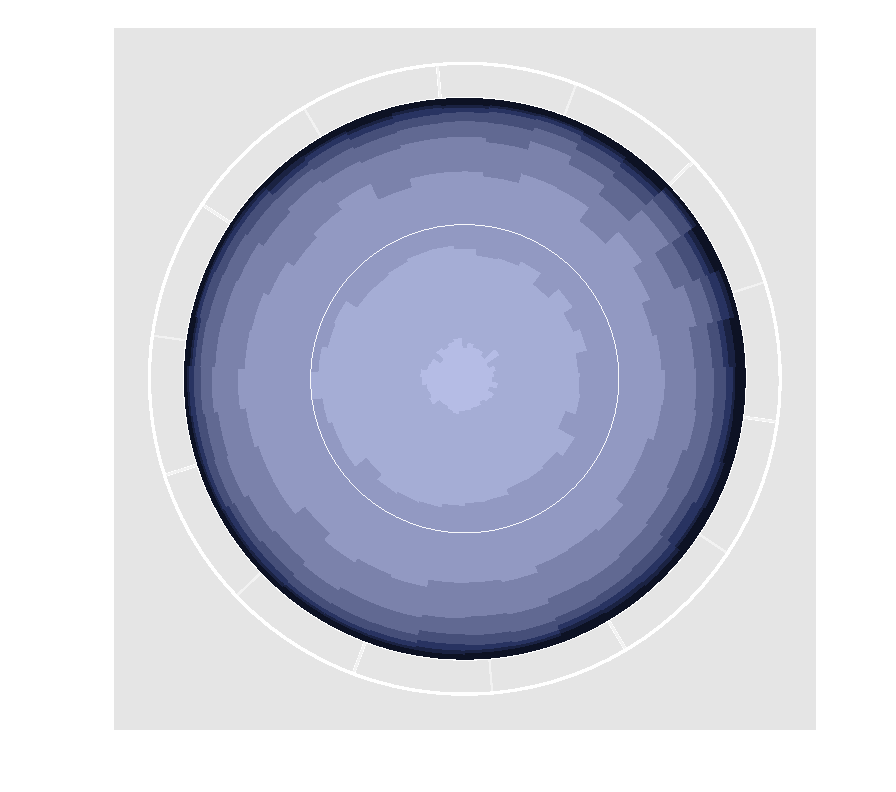
\includegraphics[width=1.3in]{Polar_Line.pdf}  
   \caption{All four layouts of charts The first row shows the data in polar coordinates and the second row shows the data in euclidian coordinates. The first column in both rows show the plots without any reference lines. The second solumn in both rows have a white reference line added. }
   \label{layouts}
\end{figure}

Amazon's Mechanical Turk is an online service in which individuals can request and perform simple tasks and surveys for money. Using Turk we were able to gather data on how people responded to the charts. Each person is shown a series of ten charts and asked to choose the graphic on each chart which they think is "different". They then identify, from a list of choices, why they chose this particular chart as well as how confident they are on a scale of one to five. Personal information such as age group, gender, and education is also collected on a voluntary basis. 

Effect is deviation from independence. Cannot be properly measured statistically except in highly aggregated situations, where the effect might be washed out.

Pie versus Barchart discussion is pretty old: cite some of the literature:

From Stephen Few, perceptual edge:
	When a graph is made, quantitative and categorical information is encoded by a display method. Then the information is visually decoded. This visual perception is a vital link. No matter how clever the choice of the information, and no matter how technologically impressive the encoding, a visualization fails if the decoding fails. Some display methods lead to efficient, accurate decoding, and others lead to inefficient, inaccurate decoding. It is only through scientific study of visual perception that informed judgments can be made about display methods. (William S. Cleveland, The Elements of Graphing Data, Hobart Press, 1994, p. 1)
	
	The systematic distortion of area is captured by �Steven�s Power Law,� which states that the psychological impression is a function of the actual physical magnitude raised to an exponent (and multiplied by a scaling constant). To be precise, the perceived area is usually equal to the actual area raised to an exponent of about 0.8, times a scaling constant...In contrast, relative line length [such as the lengths of bars] is perceived almost perfectly, provided that the lines are oriented the same way. (Kosslyn, Stephen, Graph Design for the Eye and Mind, Oxford University Press, 2006, p. 40)
	
	
	We make angle judgments when we read a pie chart, but we don�t judge angles very well. These judgments are biased; we underestimate acute angles (angles less than 90�) and overestimate obtuse angles (angles greater than 90�). Also, angles with horizontal bisectors (when the line dividing the angle in two is horizontal) appear larger than angles with vertical bisectors. (Naomi Robbins, Creating More Effective Graphs, Wiley, 2005, p. 49)
	
	 Edward Tufte once said that �the only worse design than a pie chart is several of them, for then the viewer is asked to compare quantities located in spatial disarray both within and between pies� (Edward Tufte, The Visual Display of Quantitative Information, Graphics Press, 1983, p. 178.)

 We do not claim to settle the question - which is multi-facetted and will not have a clear 'winning' design but instead very much depends on the purpose of the chart and task at hand.

\section{Results and Discussion}

\section{Conclusion}


%% if specified like this the section will be ommitted in review mode
\acknowledgments{
This work was supported in part by
NSF DMS 1007697.}

\bibliographystyle{abbrv}
%%use following if all content of bibtex file should be shown
%\nocite{*}
\bibliography{references}
\end{document}